\newpage
\section{Context: Hydrocarbon Exploration}

The processes of Reverse Time Migration and solving forward problems in creating images of the underground is primarily used in the field of hydrocarbon exploration. This relatively recent field has its origins in the 1900's, but most of the major oil pockets have already been discovered and now the job of hydrocarbon exploration becomes more difficult and necessary in underground zones that are smaller and harder to image. Add to this the difficulties of the often mountainous or forest-heavy terrain above the surface, and we can see that the hydrocarbon exploration is an increasingly complicated field in both the geophysical and mathematical domains. 

The cost of discovering a barrel has skyrocketed more than three-fold over the last decade due to these increasingly inhospitable environmental conditions and a fairly constant reduction of existing reserves at $5-15\%$ per year \cite{hydrocarbonExplorationCosts}. In addition, political risks associated with the discovery and drilling of new oil wells have been escalating. For example, the USA, Russia, Canada, Denmark, Iceland, and Norway have competing claims over the Arctic Circle where approximately a fifth of the world's recoverable oil is contained. Although Uganda has more than 2 billion barrels of oil, necessary negotiations between the government and oil companies have been slow. In 2009, 3D seismic surveys cost on average between \$40,000 and \$100,000 per square mile.

\subsection{Seismic Acquisition}

\begin{figure}[ht]
	\centering
	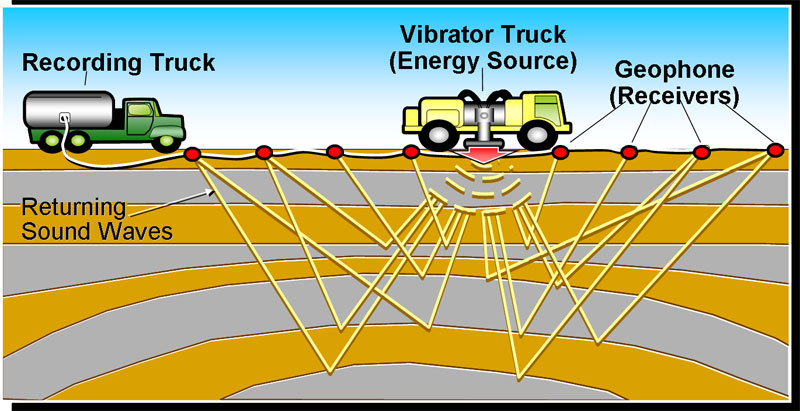
\includegraphics[width=0.39\textheight]{Images/SeismicChes5.jpg}
	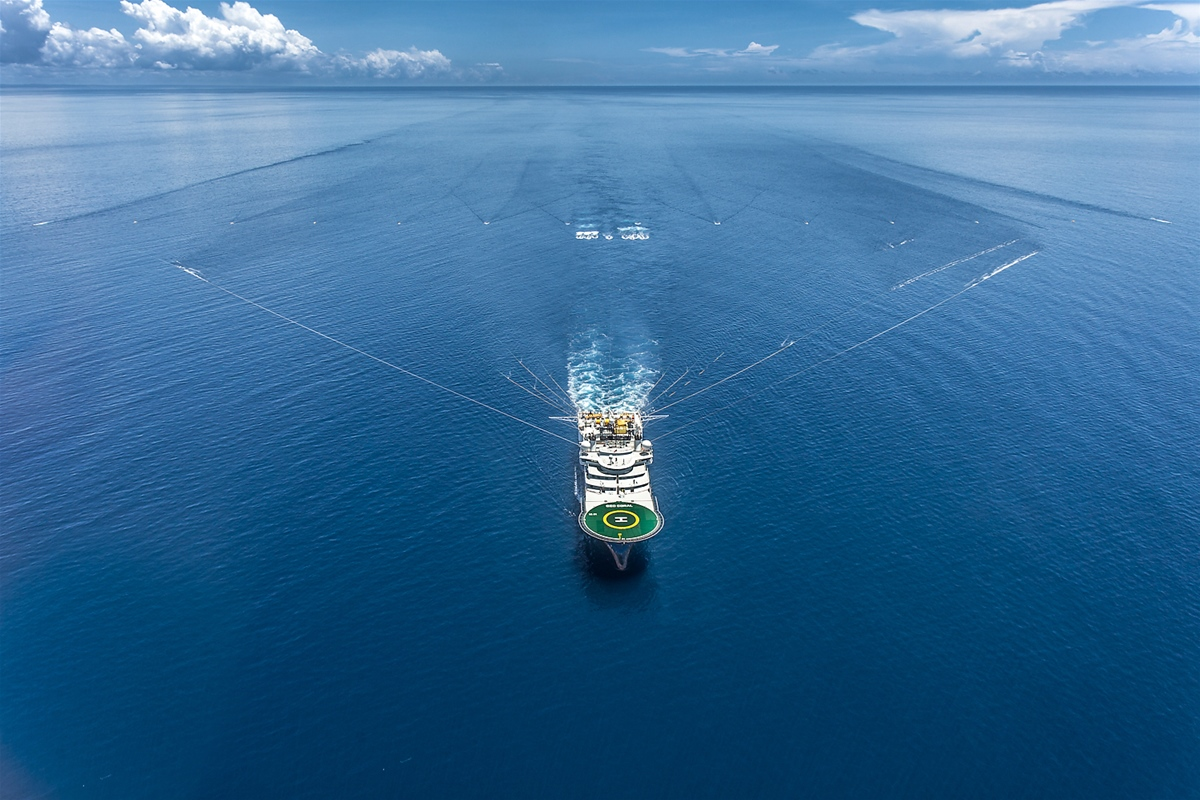
\includegraphics[width=0.3\textheight]{Images/2562_geo_coral_large.jpg}
	\caption{Model of Source and Receivers on land and maritime}
	\label{fig:Sesmic-Acquisition}
\end{figure}

In the domain of hydrocarbon exploration, there is a long and complicated sequence of data processing given the seismic surveys generated from the energy sources and receivers. The goal of this sequence of steps is to generate from the data an accurate image of the 3-dimensional interior of the earth for analysis by geophysicists. Specifically, the data consists of the measurement of energy that the receivers record over time after a signal has been sent by the source and reflected by heterogeneities within the earth.

\subsection{Method of Exploration: Seismic Reflection}


\subsection{Processing the data}


\subsection{Seismic Waves}


\subsubsection{Waves in 3D}



















